\section{HR Simulation}
\label{sec:HRsim}
The HR simulation handles all parts of the Human Resources process. Two employee types have to be hired: enigneers and salespeople. The role of HR, finance and marketing is performed by the player itself, thus it is not required to hire employees in these departments for the simulation. 

\subsection{Hiring / Firing}
The HR process starts with hiring human resources. Therefore, available engineers and salespeople need to be chosen from the market. Each employee has a requested salary. Moreover, hiring and also firing of employees is associated with cost of 5,000 CapCoins. \cite{recruiterbox}

\subsection{Salary}
Salaries are an important factor in the HR process. In order to make the simulation as realistic as possible, we use the following salaries which are derived from a salary-list of a real world IT company. The salaries of available employees are randomized value out of the corresponding salary-range entry in table \ref{tab:Salaries}

\begin{table}
    \centering
\begin{tabular}{c|c}
    \hline
     \textbf{Skilllevel} & \textbf{Salary-range in thousands cc} \\
     \hline \hline
     0-20 & 38-45  \\
     21-40 & 45-55 \\
     41-60 & 55-70  \\
     61-80 & 70-100  \\
     81-100 & 100-150  \\
     \hline

\end{tabular}
\caption{Salaries}
    \label{tab:Salaries}
\end{table}

\subsection{Key Performance Indicators}
\label{sub:KPI}
\subsubsection{Job Satisfaction}
\label{subsub:jss}
The job satisfaction is an essential part of a Key Performance Indicator framework in order to measure the management quality of the player. Many different parts in the cooperation depend on the job satisfaction of employees, thus, in order to increase the performance, managers need to make sure that the satisfaction of their employees is constantly high. \cite{KOYS}

The job satisfaction is such an important factor due to the fact that the employer branding is influenced by it. This is critical as the employer branding has a huge impact on how the company is perceived on the markets by potential employees but also by customers and suppliers. Moreover, the employer branding is also influenced by the general company image and can be influenced through marketing and PR activities. 

The success of a company highly depends on the ability of attracting the best people. The ease of recruitment is highly dependent on the job satisfaction of the employees. Extrinsic motivation needs to be provided to attract employees in case the job satisfaction and by this the employer branding are low. A low job satisfaction makes it necessary to pay higher salaries. Not only the recruiting of employees is more difficult with a lower job satisfaction but also the employee turnover is higher. A job satisfaction below 50 leads to an increase in hiring costs of 50\% which sums up to 7500 CapCoins \cite{frederiksen2016}

Different factors exist which influence the job satisfaction. \cite{Kapur} The implementation and integration of softfactors which influence the job satisfaction was not the primary goal for CapX, we concentrated on the hardfactors which include salary and paymix, worktime, the skills and education and the provided benefits by the company. 

The table \ref{tab:benefitsJSS} shows the possible influencing factors which can be chosen by the player to influence the employees job satisfaction. The monetary impact is counted in CapCoins per employee per month. 

\begin{table}
    \centering
\begin{tabular}{l|c|c}
    \hline
     \textbf{Benefit} & \textbf{Points} & \textbf{Monetary impact in cc} \\
     \hline \hline
     \multicolumn{1}{c|}{\underline{\textbf{Salary}}} & & \\
     Salary below average & 0 &  \\
     Salary on average & 2 &  \\
     Salary above average & 4 &   \\
     \hline
     \multicolumn{1}{c|}{\underline{\textbf{Working Time Model}}} & & \\
     Fixed Model & 0 &   \\
     Flextime model & 1 &   \\
     Trust-based (TB) & 2 &   \\
     Trust-based (TB) + HO once a week & 3 &   \\
     Trust-based (TB) + always HO allowed & 4 &   \\
     \hline
     \multicolumn{1}{c|}{\underline{\textbf{Worktime}}} & & \\
     10 hours & 0 & 0  \\
     8 hours & 3 & 0  \\
     6 hours & 5 & -1000  \\
     \hline
     \multicolumn{1}{c|}{\underline{\textbf{Company Car}}} & & \\
     Not offered & 0 & 0  \\
     Medium Size & 2 & -300  \\
     Full Size & 4 & -600  \\
     \hline
     \multicolumn{1}{c|}{\underline{\textbf{IT Equipment}}} & & \\
     Market Average & 0 & 0  \\
     High End & 2 & -50  \\
     \hline
     \multicolumn{1}{c|}{\underline{\textbf{Food / Coffee}}} & & \\
     Employee payment & 0 & 0  \\
     Offered for free & 4 & -100  \\
     \hline
     \multicolumn{1}{c|}{\underline{\textbf{Gym / Sports}}} & & \\
     Not offered & 0 & 0  \\
     Subsidized & 2 & -40 \\
     Offered for free & 4 & -100  \\
     \hline

\end{tabular}
\caption{Benefits influencing the Job Satisfaction}
    \label{tab:benefitsJSS}
\end{table}

For each of the above mentioned categories (salary, worktime, company car, homeoffice, IT equipment, food and sports) the player needs to make a decision which benefit category to offer. The job satisfaction score can have a minimum of 0 points and a maximum of 28 points.

As this scale is too simple in order to be somehow realistic, a manipulation of the original scale is needed. The marginal impact of an additional increase of factors which lead to a higher job satisfaction decreases over time, e.g. an employee which has an above average salary, a company car, trusted based working hours and all other benefits on the highest level, would not value the additional offering of a free sports club voucher as much as an employee that has no benefits at all and gets a sports club voucher. Thus the scale of 0 - 28 was transformed to a root function.

Moreover, the job satisfaction also depends on the level of the employee. Each employee has its own specific requirements and expectations. Generally, we assume that employees with a lower skill level, are more easily satisfied than employees with a higher skilllevel. In this case the skilllevel  is used as a proxy for the expectations of an employee towards the employer. 

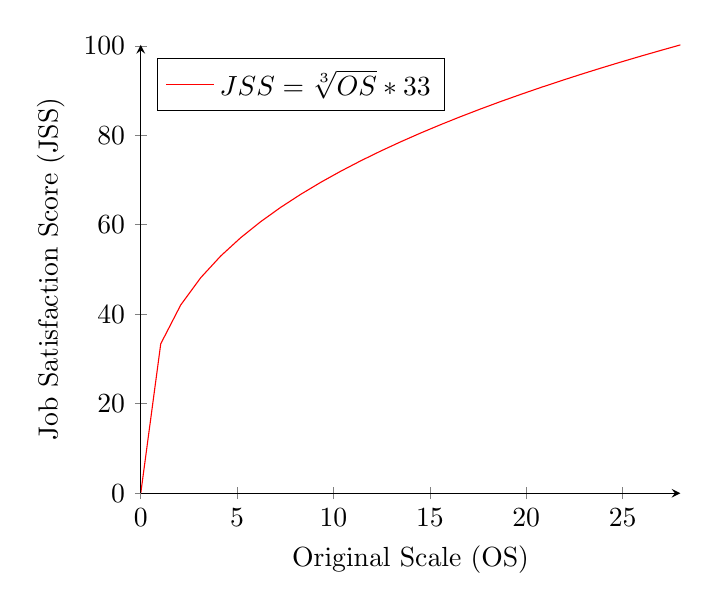
\begin{tikzpicture}
\begin{axis}[
    axis lines = left,
    xlabel = Original Scale (OS),
    ylabel = Job Satisfaction Score (JSS),
    grid style = dashed,
    legend pos=north west
]

\addplot [
    domain=0:28, 
    samples=28, 
    color=red,
]
{x^(1/3) * 33};
\addlegendentry{$JSS=\sqrt[3]{OS}*33$}
\end{axis}
\end{tikzpicture}

\subsubsection{Quality of Work}
The quality of work is a measure for the output quality of every process step in the corporation where an employee is involved. We are aware, that the quality of process outputs is influenced by more than the chosen factors here. However, for the sake of the realization of the game, we concentrated on the factors which can be chosen by a player simulating the role of a CEO or Chief Human Resources Officer (CHRO). Besides the influencing factors, which are defined and explained below, the skill level is the most important factor for the quality of an employee. The underlying assumption is that higher skilled employees have more experience and perform similar activities better than employees with a lower skilllevel in a comparable position.

The skilllevel becomes a strategic mechanism as it influences the quality of work significantly. In fact, a better quality of work leads to higher output of the production, can decrease product failure and improve the quality of the products, allows new products to be developed, and for example in case of sales employees generate more sales. 

The skilllevel alone is not enough to describe the influence on the Quality of work. The happiness and satisfaction with the job is also a measure that influences the quality of the delivered work by the employees.
Thus, the total quality of work is measured by an equal weighted average of the skilllevel and the job satisfaction. The skilllevel of employees can be influenced by trainings which is described in the section below.

\subsubsection{Training}
Employees can be categorized into 5 groups:
\begin{itemize}
    \item Worker (20)
    \item Student (30)
    \item Graduate (40)
    \item Specialist (60)
    \item Expert (80)
\end{itemize}
The initial skill level for these employees is set to (20, 30, 40, 60, 80) according to the order of the list above. In order to improve the skilllevel and by this the quality of work of the employees, training can be added to the learning journey of employees. 

Training can be assigned to a certain number of employees. The cost per training and also the increase of the skill level of the single employee depends on the kind of training. There are two different training types: courses and workshops. Both training types influence the skilllevel of the employee and the salary of the employee. The  table \ref{tab:trainings_employees} shows the impact of trainings on the salary and the skilllevel of employees.

\begin{table}
    \centering
\begin{tabular}{c|c|c}
    \hline
     & \textbf{Courses} & \textbf{Workshops} \\
     \hline \hline
     Price & 3000 cc & 5500 cc \\
     Salary & +1\% & +2\%  \\
     Skilllevel & +1 & +2  \\
     \hline
\end{tabular}
\caption{Influence of trainings on employees}
    \label{tab:trainings_employees}
\end{table}


\subsection{Summary}

The single KPIs are calculated as follows: 
% This needs to be formatted
\begin{itemize}
\item Quality of Work = $JSS \cdot 0.5 + SkillLevel \cdot 0.5$
\item Skill Level = Initial Skill Level (based on employee category + influence training
\item Job Satisfaction Score (JSS) = Calculation based on JSS section \ref{subsub:jss}
\item Company Image Score (CIS) = Calculation based on CIS section \ref{company_image}
\item Employer Branding = $JSS \cdot 0.6 + CIS \cdot 0.4$ and applying the punishment function. 
\end{itemize}